\documentclass[pdf]{beamer}
\mode<presentation>{}

\newcommand\blfootnote[1]{%
\begingroup
\renewcommand\thefootnote{}\footnote{#1}%
\addtocounter{footnote}{-1}%
\endgroup
}

\usepackage[absolute, overlay]{textpos}
\usepackage[style=verbose-ibid,backend=bibtex]{biblatex}
\bibliography{references}

\title{Layer-skipping connections facilitate training of layered networks using equilibrium propagation.}
\author{Jimmy Gammell \and Sae Woo Nam \and Adam N. McCaughan}
\date{July 28, 2020}

\begin{document}

\section{Title} % Total slide count: 7-12 slides
\begin{frame} % title slide
	\titlepage
\end{frame}

\begin{frame}
\frametitle{Motivation}
\begin{itemize}
	\item<1-> Seek to implement deep learning in neuromorphic analog hardware
	\item<2-> Want learning framework requiring simple hardware
	\begin{itemize}
		\item<3-> Neurons and connections perform few distinct tasks
	\end{itemize}
\end{itemize}
\end{frame}

\begin{frame}
\frametitle{Background: equilibrium propagation}
\begin{columns}
	\begin{column}{.5\textwidth}
		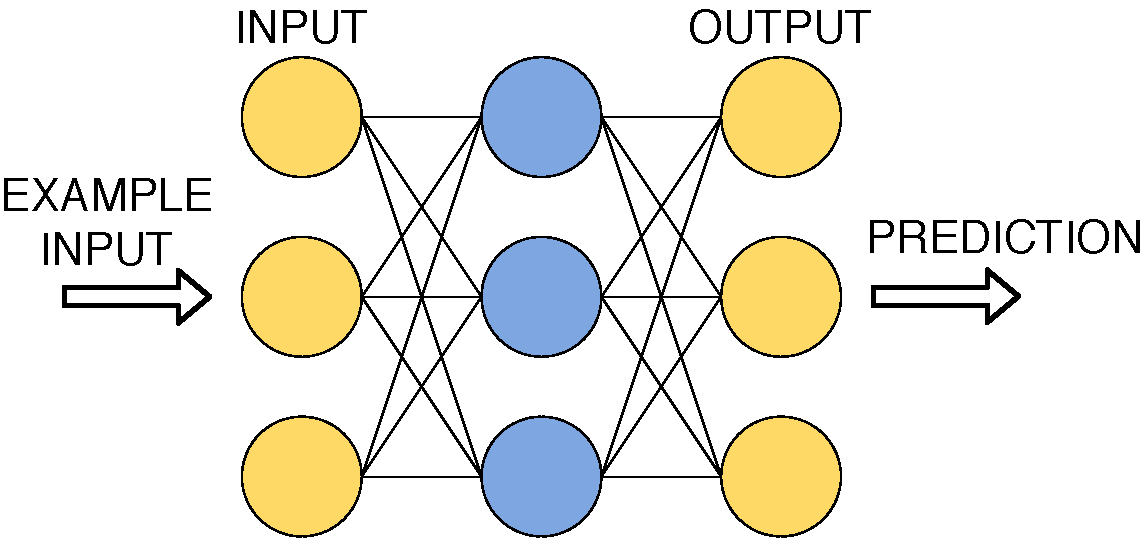
\includegraphics[width=\textwidth]{figures/eqp_free_illustration.pdf}
	\end{column}
	\begin{column}{.5\textwidth}
		\begin{itemize}
			\item<1-> Equilibrium propagation: a biologically motivated learning framework
			\begin{itemize}
				\item<2-> Gradient descent on cost function (alternative to backpropagation)
				\item<3-> Energy-based networks, e.g. continuous Hopfield network
			\end{itemize}
			\item<4-> First phase of training: free phase
			\begin{itemize}
				\item<5-> Evolve to equilibrium for input
				\item<6-> Prediction: output activations at equilibrium
			\end{itemize}
		\end{itemize}
	\end{column}
\end{columns}
\blfootnote{Scellier and Bengio, Equilibrium Propagation: Bridging the Gap Between Energy-Based Models and Backpropagation}
\end{frame}

\begin{frame}
\frametitle{Background: equilibrium propagation}
\begin{columns}
	\begin{column}{.5\textwidth}
		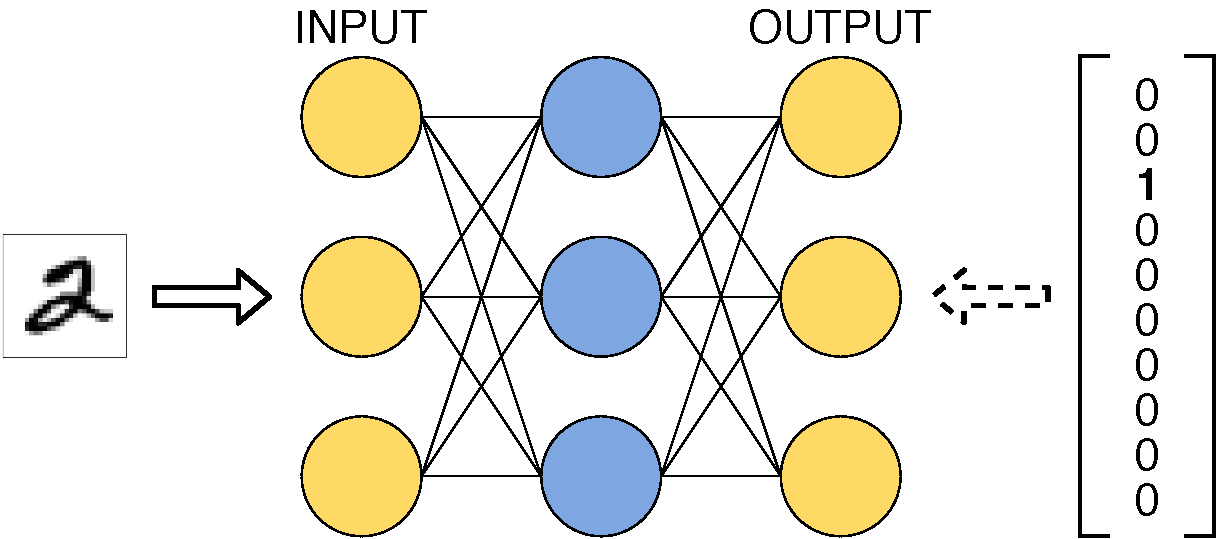
\includegraphics[width=\textwidth]{figures/eqp_weakly_clamped.pdf}
	\end{column}
	\begin{column}{.5\textwidth}
		\begin{itemize}
			\item<1-> Second phase of training: weakly-clamped phase
			\begin{itemize}
				\item<2-> Perturb output activations towards target output
				\item<3-> Evolve to equilibrium
			\end{itemize}
			\item<4-> Differences between equilibrium states can be used to compute gradient
		\end{itemize}
	\end{column}
\end{columns}
\end{frame}

\begin{frame}
\frametitle{Background: equilibrium propagation}
\begin{itemize}
	\item<1-> Advantageous due to simplicity of neurons and connections
	\begin{itemize}
		\item<2-> One computation in both phases of training
		\item<3-> One type of information to transmit in both phases of training
		\item<4-> Biologically-plausible (relative to backpropagation)
		\item<5-> Implementable in neuromorphic analog hardware
	\end{itemize}
\end{itemize}
\end{frame}

\begin{frame}
\frametitle{Background: vanishing gradient problem}
\begin{columns}
	\begin{column}{.5\textwidth}
		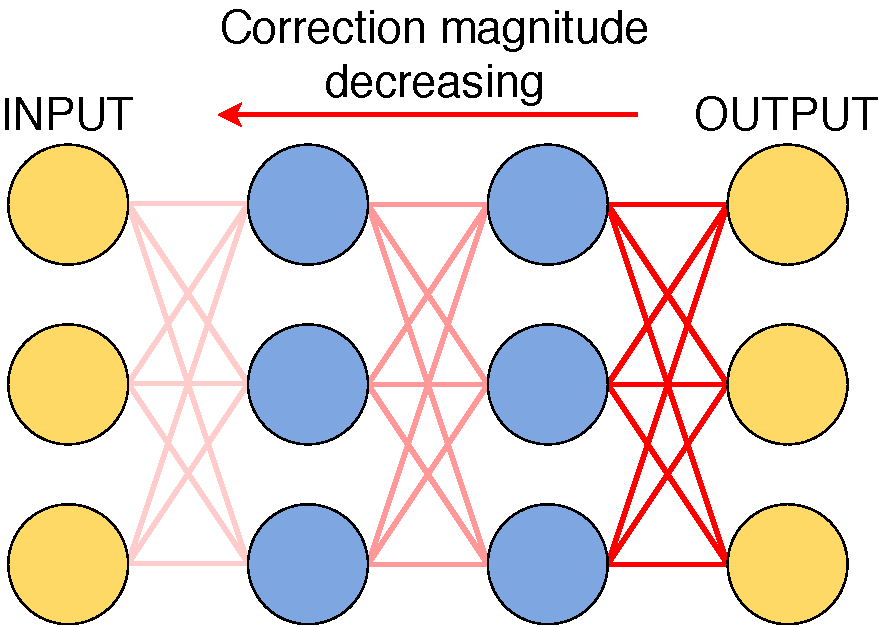
\includegraphics[width=\textwidth]{figures/vgp_illustration.pdf}
	\end{column}
	\begin{column}{.5\textwidth}
		\begin{itemize}
			\item<1-> Problem: vanishing gradients in layered networks
			\vspace{-4mm}\begin{itemize}
				\item<2-> Slow training
				\item<3-> Bit-depth issues
			\end{itemize}
			\item<4-> Need to solve - deep networks better than shallow networks
			\item<5-> Not yet solved in simple, biologically-plausible manner
		\end{itemize}
	\end{column}
\end{columns}
\end{frame}

\begin{frame}
\frametitle{Background: vanishing gradient problem}
\begin{columns}
	\begin{column}{.5\textwidth}
		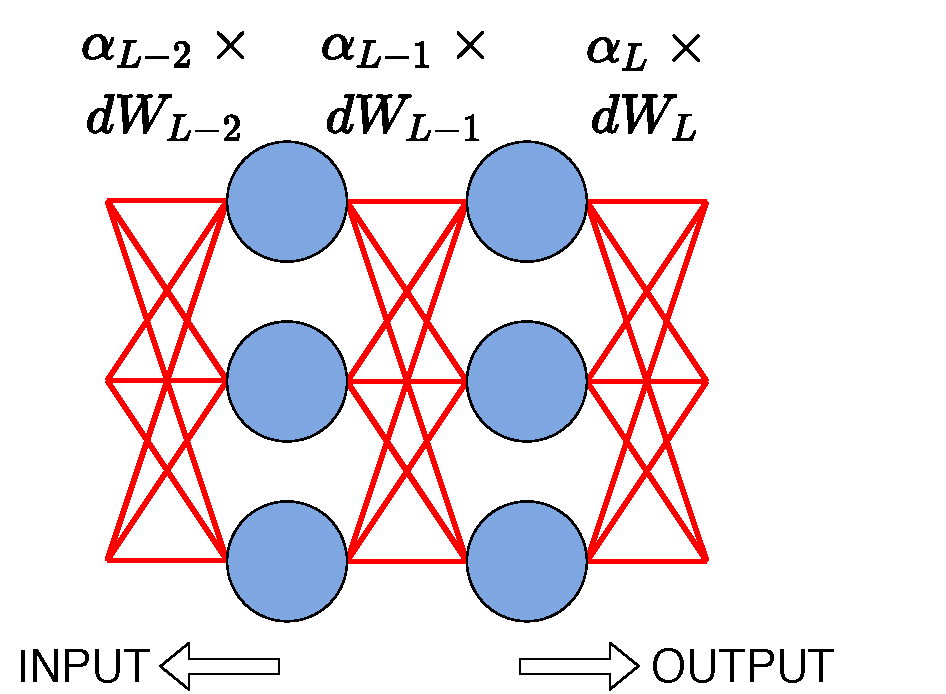
\includegraphics[width=\textwidth]{figures/perlayer_illustration.pdf}
	\end{column}
	\begin{column}{.5\textwidth}
		\begin{itemize}
			\item<1-> Original paper: independent learning rates for each layer
			\begin{itemize}
				\item<2-> Increase with depth to compensate
			\end{itemize}
			\item<3-> Unappealing for following reasons:
			\begin{enumerate}
				\item<4-> More hyperparameters to tune
				\item<5-> Inconvenient in neuromorphic hardware
				\item<6-> Seems unlikely in biological systems
			\end{enumerate}
			\item<7-> Problem can be mitigated by instead using topological modification based on layer-skipping connections
		\end{itemize}
	\end{column}
\end{columns}
\end{frame}

\begin{frame}
\frametitle{Our solution: layer-skipping connections}
\begin{itemize}
	\item<1-> Vanishing gradient problem can be mitigated with layer-skipping connections
	\item<2-> Topology inspired by small-world networks
\end{itemize}
\end{frame}

\section{Solution}

\subsection{Original topology illustration}
\begin{frame}
	\frametitle{Original layered topology}
	\begin{columns}
	\begin{column}{.6\textwidth}
		\begin{center}
		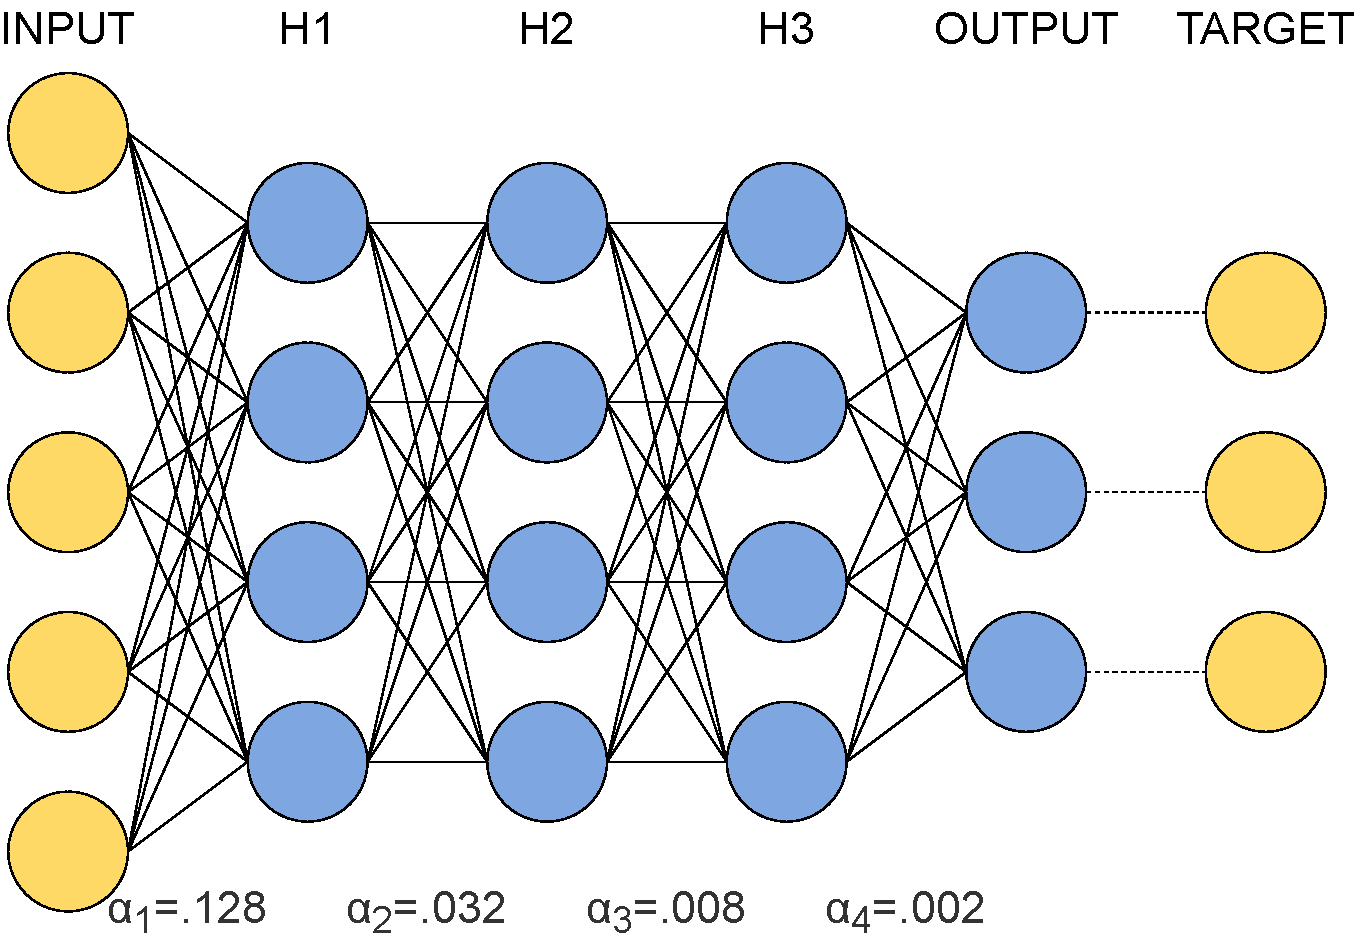
\includegraphics[width=\textwidth]{figures/basic_topology_illustration.pdf}
		\end{center}
	\end{column}
	\begin{column}{.4\textwidth}
		\begin{itemize}
			\item From original paper
			\item Per-layer learning rates
		\end{itemize}
	\end{column}
	\end{columns}
\end{frame}

\begin{frame}
	\frametitle{Our topological modifications}
	\begin{columns}
		\begin{column}{.6\textwidth}
			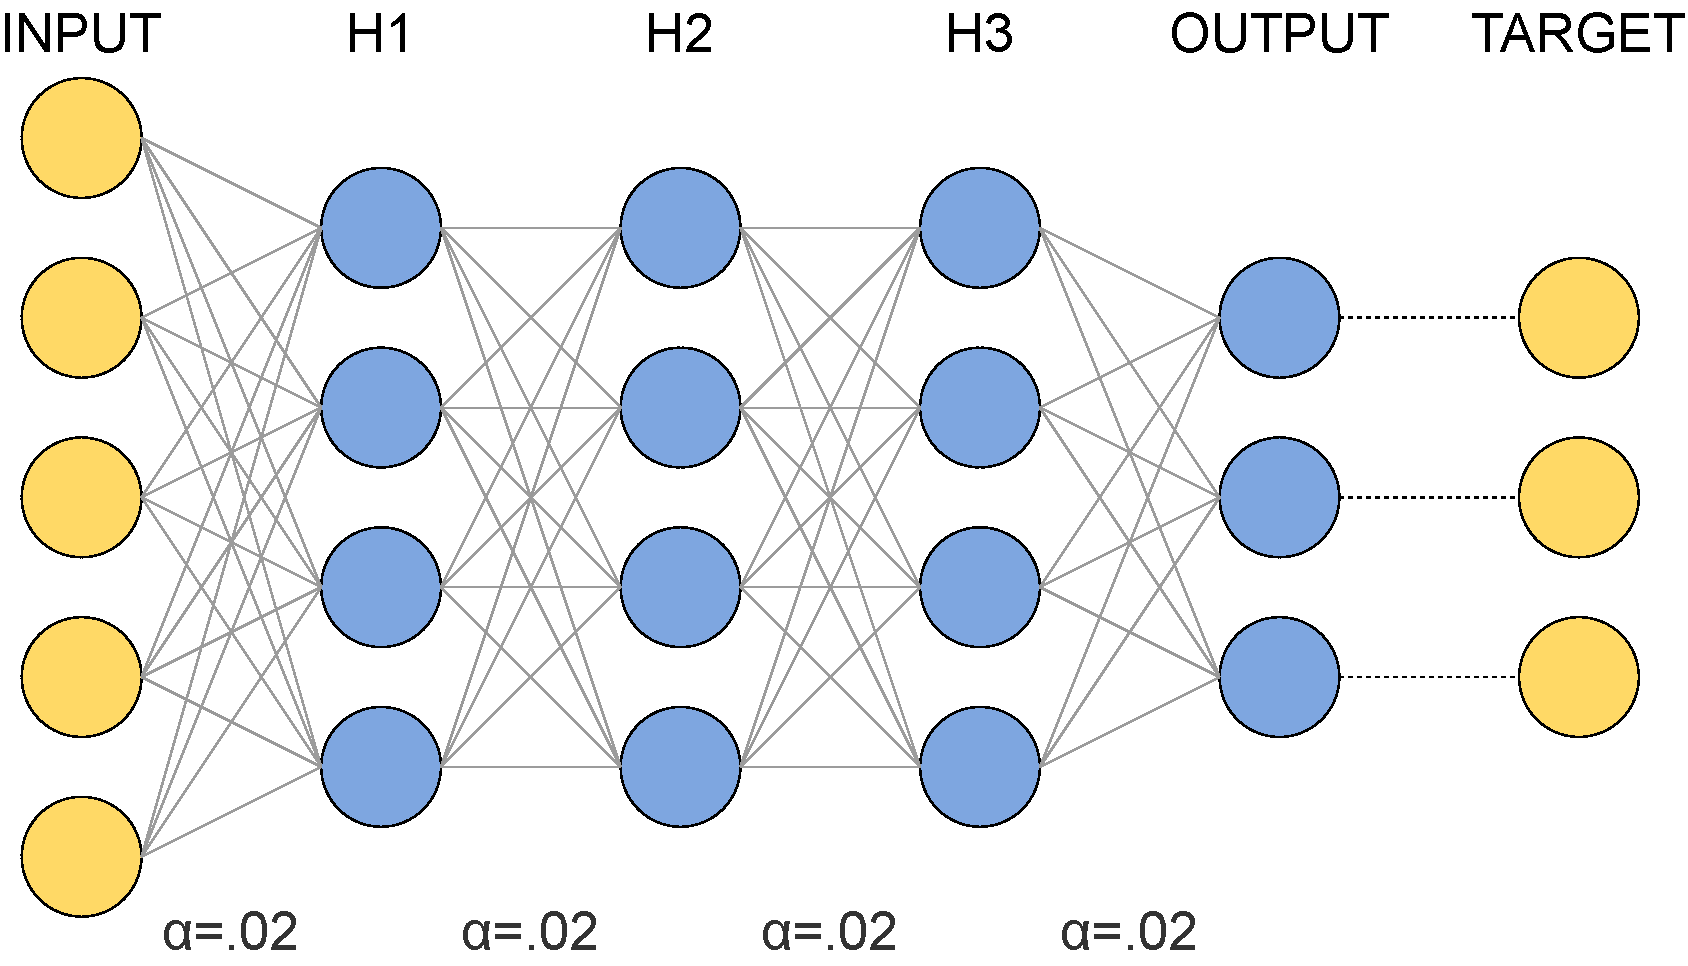
\includegraphics[width=\textwidth]{figures/topology_changes_step1.pdf}
		\end{column}
		\begin{column}{.4\textwidth}
			\begin{itemize}
			\item Starting point: original topology
			\item One learning rate for all layers
			\end{itemize}
		\end{column}
	\end{columns}
\end{frame}
\begin{frame}
	\frametitle{Our topological modifications}
	\begin{columns}
		\begin{column}{.6\textwidth}
			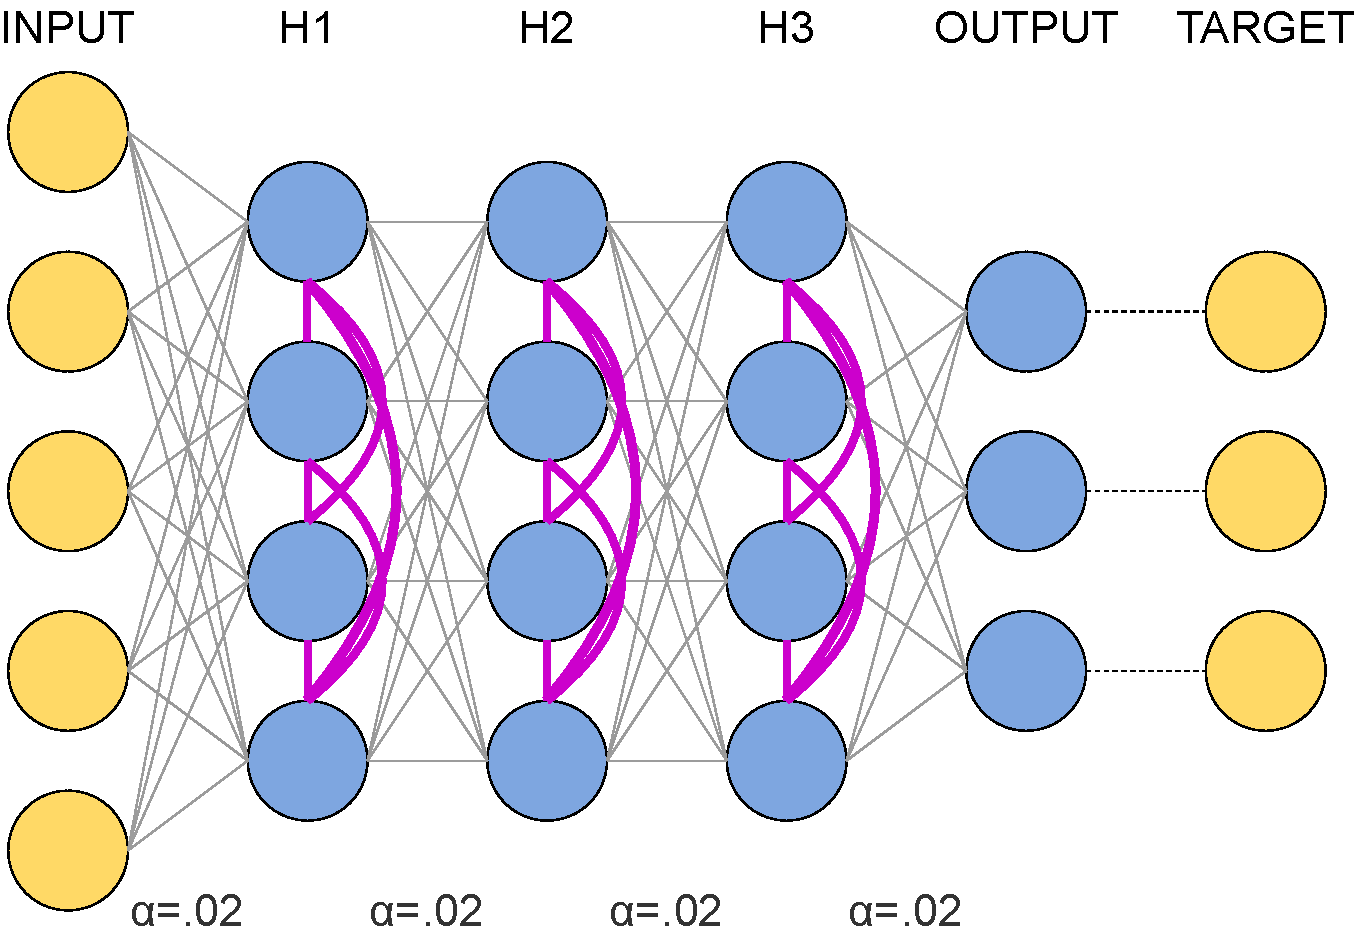
\includegraphics[width=\textwidth]{figures/topology_changes_step2.pdf}
		\end{column}
		\begin{column}{.4\textwidth}
			\begin{itemize}
			\item Hidden layers fully connected
			\end{itemize}
		\end{column}
	\end{columns}
\end{frame}
\begin{frame}
	\frametitle{Our topological modifications}
	\begin{columns}
		\begin{column}{.6\textwidth}
			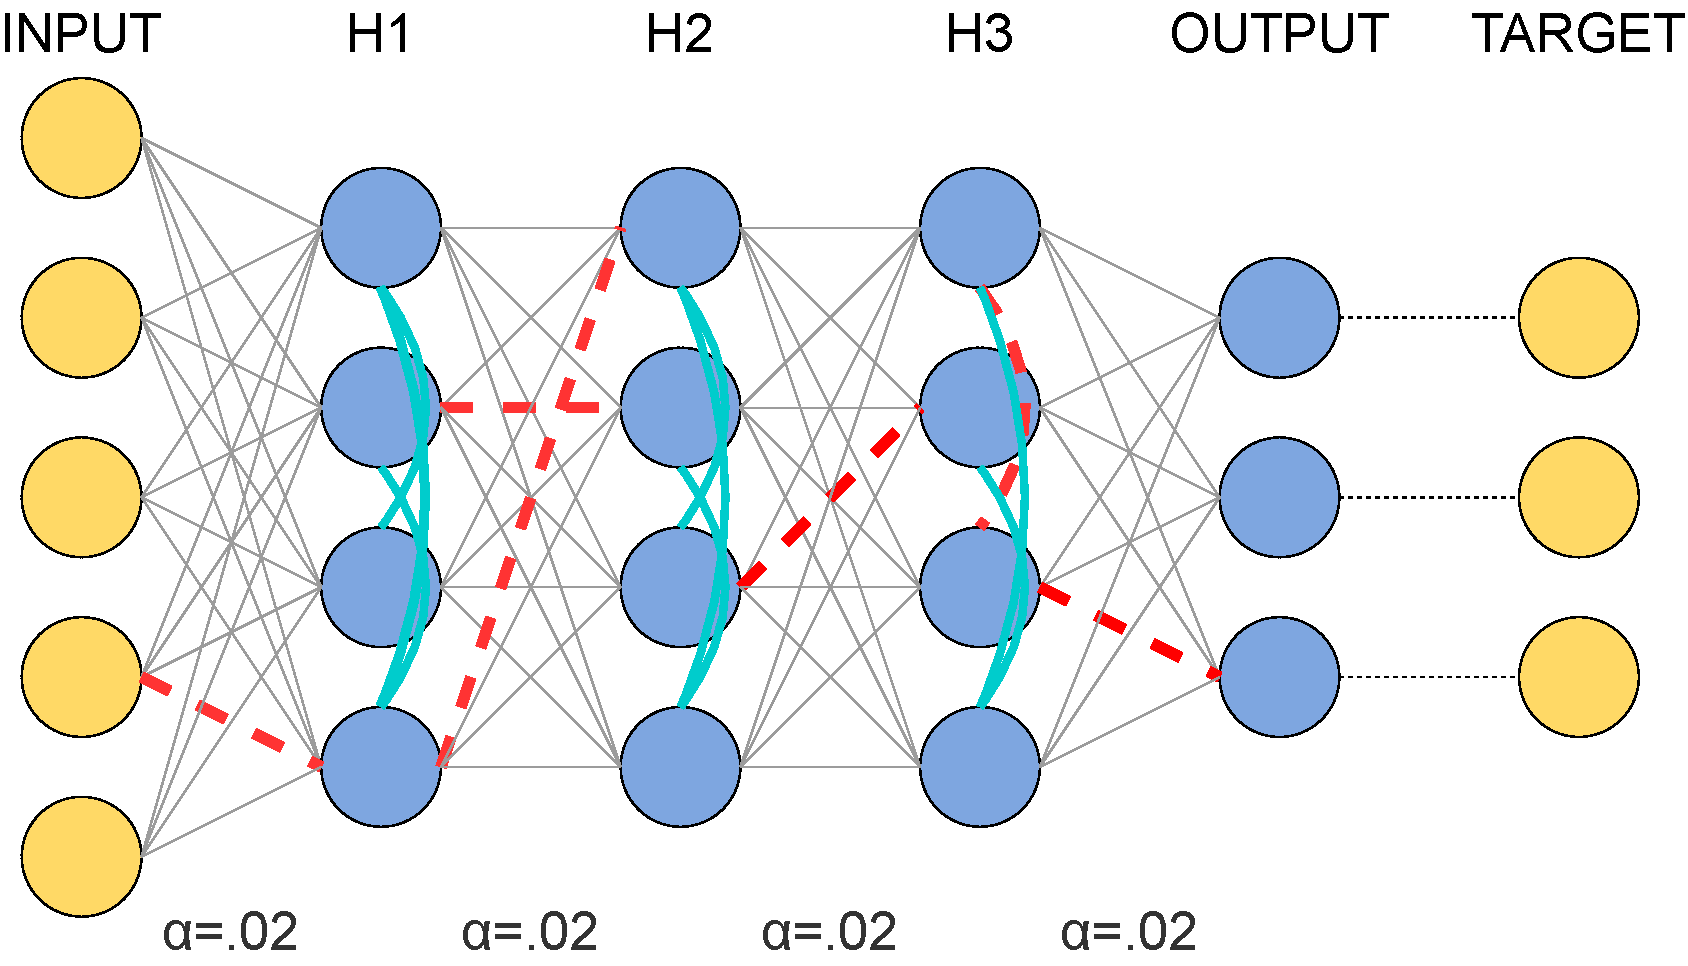
\includegraphics[width=\textwidth]{figures/topology_changes_step3.pdf}
		\end{column}
		\begin{column}{.4\textwidth}
			\begin{itemize}
			\item Consider each connection
			\item Remove with probability $p$
			\end{itemize}
		\end{column}
	\end{columns}
\end{frame}
\begin{frame}
	\frametitle{Our topological modifications}
	\begin{columns}
		\begin{column}{.6\textwidth}
			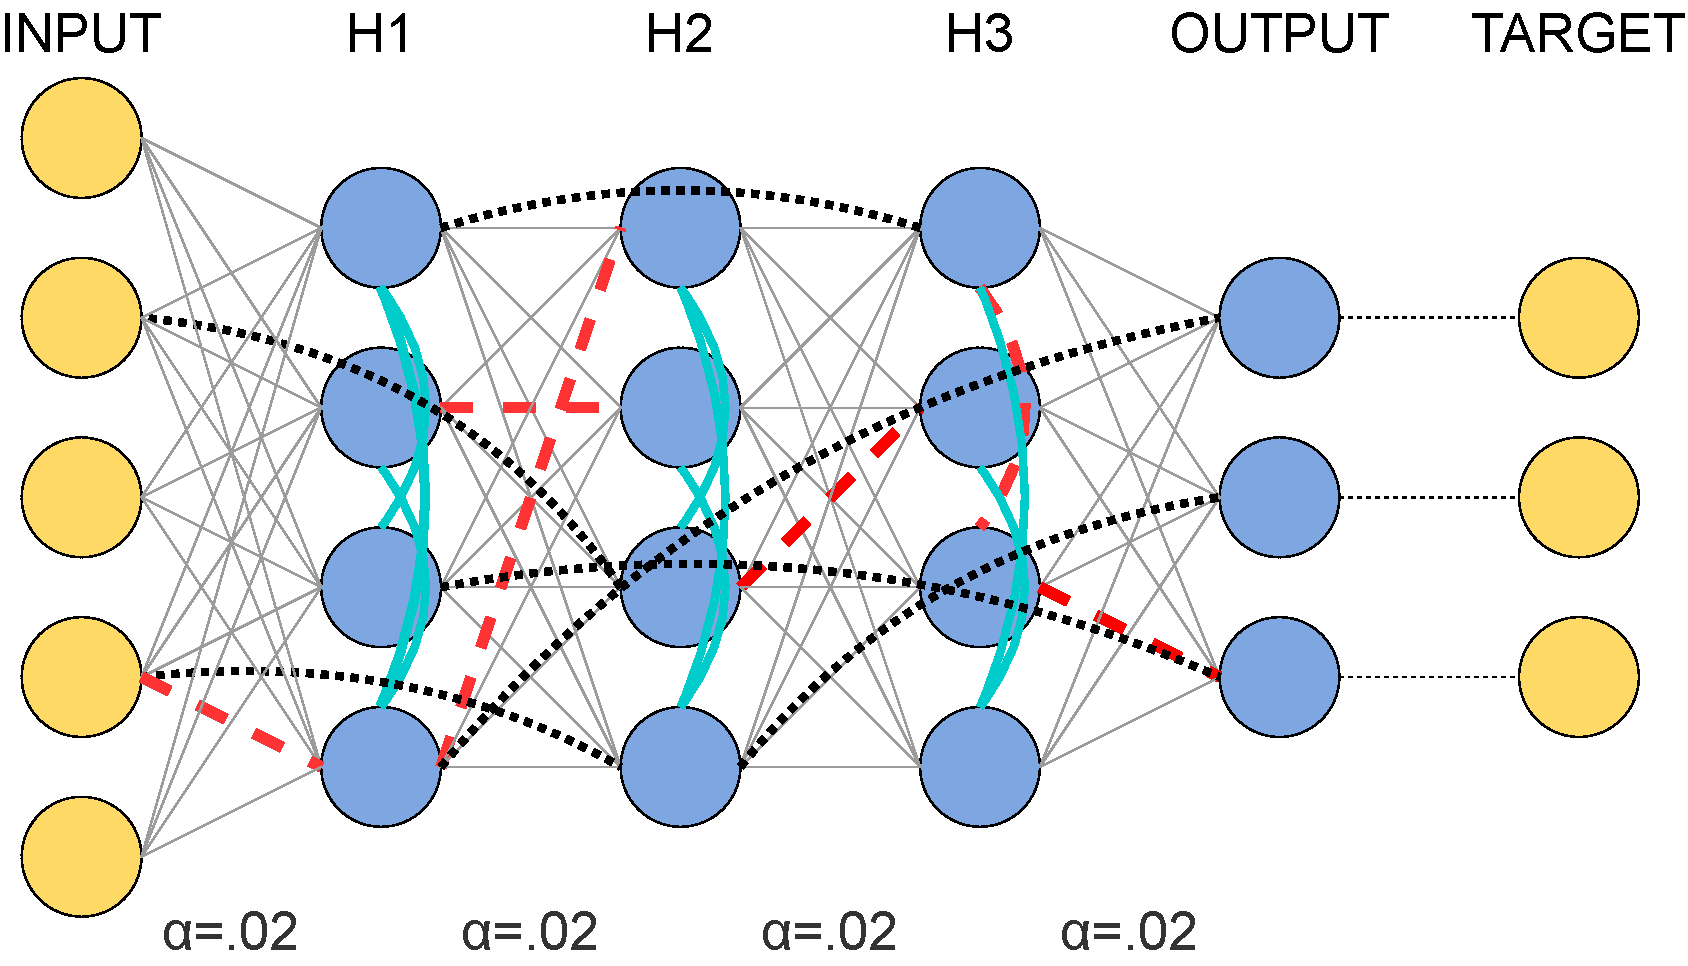
\includegraphics[width=\textwidth]{figures/topology_changes_step4.pdf}
		\end{column}
		\begin{column}{.4\textwidth}
			\begin{itemize}
			\item For each removed connection, randomly connect a different pair
			\item No connections within input or output layers
			\end{itemize}
		\end{column}
	\end{columns}
\end{frame}

\section{Results}
\subsection{Performance comparison between topologies}
\begin{frame}
	\frametitle{Results: training error of layered network with per-layer learning rates}
	\begin{columns}
	\begin{column}{.6\textwidth}
		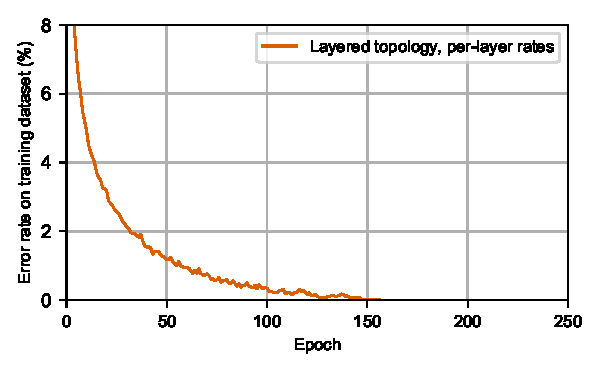
\includegraphics[width=\textwidth]{figures/performance_original.pdf}
	\end{column}
	\begin{column}{.4\textwidth}
	\begin{itemize}
		\item Baseline performance: network from original paper
		\item Per-layer learning rates
	\end{itemize}
	\end{column}
	\end{columns}
\end{frame}
\begin{frame}
	\frametitle{Results: training error of layered network with single global learning rate}
	\begin{columns}
	\begin{column}{.6\textwidth}
		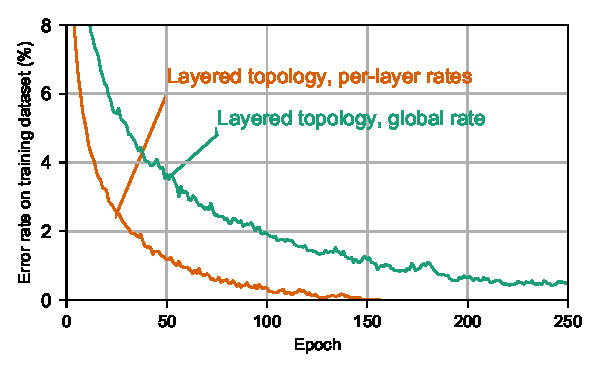
\includegraphics[width=\textwidth]{figures/performance_original+global.pdf}
	\end{column}
	\begin{column}{.4\textwidth}
	\begin{itemize}
		\item Network with one global learning rate
		\item Training slows down
	\end{itemize}
	\end{column}
	\end{columns}
\end{frame}
\begin{frame}
	\frametitle{Results: training error of network with our topology}
	\begin{columns}
	\begin{column}{.6\textwidth}
		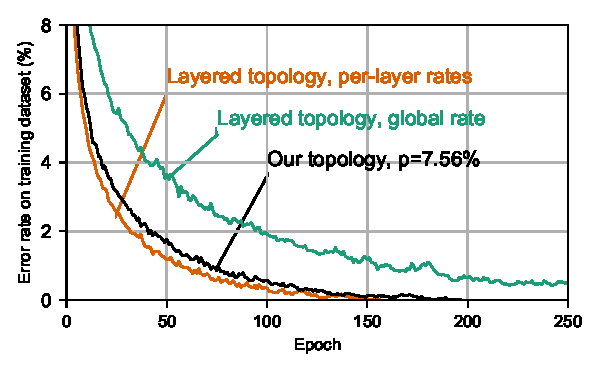
\includegraphics[width=\textwidth]{figures/performance_original+global+ours.pdf}
	\end{column}
	\begin{column}{.4\textwidth}
	\begin{itemize}
		\item Network with our topology (still one global learning rate)
		\item Trains significantly faster than layered network
		\item Performance similar to original network
	\end{itemize}
	\end{column}
	\end{columns}
\end{frame}
\subsection{Layer training rate comparison between topologies}
\begin{frame}
	\frametitle{Results: vanishing gradient in layered network with single global learning rate}
	\begin{columns}
	\begin{column}{.6\textwidth}
		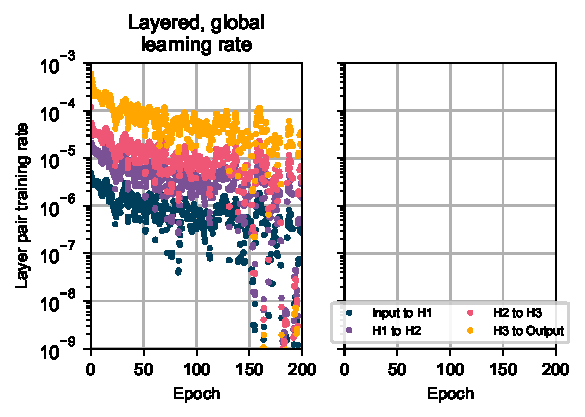
\includegraphics[width=\textwidth]{figures/perlayer_global.pdf}
	\end{column}
	\begin{column}{.4\textwidth}
		\begin{itemize}
			\item Vanishing gradient problem when one learning rate is used
		\end{itemize}
	\end{column}
	\end{columns}
\end{frame}
\begin{frame}
	\frametitle{Results: vanishing gradient in layered network with our topology}
	\begin{columns}
	\begin{column}{.6\textwidth}
		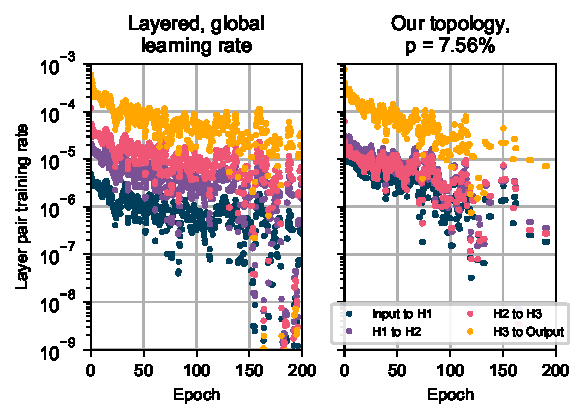
\includegraphics[width=\textwidth]{figures/perlayer_global+ours.pdf}
	\end{column}
	\begin{column}{.4\textwidth}
		\begin{itemize}
			\item<1-> Our topology mitigates vanishing gradient problem
			\item<2-> Shallowest weights train faster due to lack of layer-skipping connections to target
		\end{itemize}
	\end{column}
	\end{columns}
\end{frame}

\begin{frame}
	\frametitle{Conclusions}
	\begin{itemize}
		\item<1-> Our topology mitigates vanishing gradient problem
		\item<2-> Avoids issues with per-layer rates
		\begin{enumerate}
			\item<3-> Only two new hyperparameters; constant with depth
			\item<4-> Small-world networks have been observed in biological brains
			\item<5-> Easy to implement in networks with configurable connectivity
		\end{enumerate}
		\item<6-> Good solution where simplicity, biological plausibility important
	\end{itemize}
\end{frame}

\section{Directions for future research}
\begin{frame}
	\frametitle{Directions for future research}
	\begin{itemize}
		\item<1-> Try on harder datasets (e.g. CIFAR, ImageNet) where depth is very important
		\item<2-> Effect of $p$ on test error
		\item<3-> Effectiveness on deeper networks
		\item<4-> Try training a network with added layer-skipping connections, then removing them afterwards
	\end{itemize}
\end{frame}

\section{Acknowledgments}
\begin{frame}
\frametitle{Acknowledgments}
\begin{columns}
\begin{column}{.48\textwidth}
	\begin{itemize}
		\item Sonia Buckley
		\item Zach Grey
		\item Adam N. McCaughan
		\item Sae Woo Nam
		\item Alex Tait
	\end{itemize}
\end{column}
\begin{column}{.48\textwidth}
	
\includegraphics[width=.8\textwidth]{figures/nist_logo.png}
	\\\vspace{.5cm}
	
\includegraphics[width=.8\textwidth]{figures/cu_logo.jpg}
\end{column}
\end{columns}
\end{frame}

\end{document}